
\section{Geometría afín (salto al tema 11)}

Dejamos el mundo abstracto de las estructuras algebraicas para empezar con la geometría. 

El planeta tierra existe antes de que se inventen las coordenadas GPS. 


Lo que vamos a hacer es determinar las "coordenadas GPS" de todos los puntos del espacio tridimensional.
%
Para ello, necesitaremos tener un sistema de referencia consensuado.
%
Así, fijando un sistema de referencia, podemos empezar a trabajar con elementos que se encuentren en algún lugar de algún espacio. 



\begin{defn}[Sistema de referencia] (Página 277)
Sea $V$ un espacio vectorial con base $\mathcal{B}$ y sea $O$ un punto, que llamaremos \textbf{origen de coordenadas}

Llamamos Sistema de referencia afín al conjunto $S = \{\mathcal{B},O\}$
\end{defn}

\begin{example}
En el sistema de referencia $S=\{O = (1,2,3); \mathcal{B} = \{\vec{u_1} = (1,1,1), \vec{u_2} = (2,1,0), \vec{u_3} = (0,0,1)\}\}$

En este sistema de referencia, $\vec{a} = (2,7,3)$ significa:

$\vec{a} =  (1,2,3) + 2\cdot u_1 + 7\cdot u_2 + 3\cdot u_3$ si quisiéramos escribirlo en función del sistema de referencia habitual.

\label{example::origen_ref}

Si se va a trabajar y a hacer operaciones siempre con el mismo sistema de referencia, con origen $(1,2,3)$, trabajaremos con $\vec{a} = 2\cdot u_1 + 7\cdot u_2 + 3\cdot u_3$.
%
Al final, uno puede prácticamente ignorar el origen, trabajar como si fuera otro y despues sumar o restar para corregir el punto de origen.

\end{example}
\obs En el ejemplo anterior, se ha realizado la operación: $\vec{a} =  (1,2,3) + 2·u_1 + 7·u_2 + 3·u_3$. \ul{¿Cómo se suman puntos y vectores?} 
%
No es posible sumar puntos con vectores (como no es posible sumar peras con manzanas). La manera de hacer esta operaciónes considerar $(1,2,3)$ como un vector al que llamaremos vector de posición.


Un sistema de referencia permite definir \concept[Vector\IS de posición]{vectores de posición} para situar los puntos unívocamente en el espacio.
%
El vector de posición $\vec{OP}$ es el vector que une el punto $P$ con el punto $O$, origen de coordenadas. 
%
La \textbf{ventaja de los vectores de posición} es que permiten hacer operaciones, ya que \ul{\textbf{los puntos no se pueden sumar}}.



\begin{problem}

Dado el sistema de referencia $S_1=\{O = (0,0,0); \mathcal{B} = \{\vec{i},\vec{j},\vec{k}\}\}$

\ppart Si $\vec{a} = (13,1,-5)$ está expresado en función de $S_1$, halla sus coordenadas en $S_2=\{O = (0,1,-5); \mathcal{B} = \{\vec{i},\vec{j},\vec{k}\}\}$

\ppart Haz el mismo ejercicio, tomando $S_1=\{O = (1,2,3); \mathcal{B} = \{\vec{i},\vec{j},\vec{k}\}\}$

\solution
\hide{
\spart 
\[
  \vec{a} = (13,1,-5) = (0,1,-5) + \lambda_1\vec{i} + \lambda_2\vec{j} + \lambda_3\vec{k} \dimplies \left\{
    \begin{array}{c}
      13 = \lambda_1\\
      1 = 1 + \lambda_2\\
      -5 = -5 + \lambda_3
    \end{array}
  \right\} \]
\[\dimplies (\lambda_1,\lambda_2,\lambda_3) = (13,0,0)
\]

\spart 
En realidad, $\vec{a}$ sería el vector de posición del punto $(14,3,-2)$, teniendo en cuenta que $O(1,2,3)$, por lo que:
\[
  \vec{a} = (14,3,-2) = (0,1,-5) + \lambda_1\vec{i} + \lambda_2\vec{j} + \lambda_3\vec{k} \dimplies \left\{
    \begin{array}{c}
      14 = \lambda_1\\
      3 = 1 + \lambda_2\\
      -2 = -5 + \lambda_3
    \end{array}
  \right\} \]
\[\dimplies (\lambda_1,\lambda_2,\lambda_3) = (14,2,3)
\]
}


\end{problem}


\obs Ya tenemos un sistema de referencia para movernos entre puntos. 
%
Habitualmente trabajaremos con $S= \{O(0,0,0), \mathcal{B} = \{(1,0,0), (0,1,0), (0,0,1)\}\}$ como sistema de referencia de $\mathcal{V}^3$.



\paragraph{Vectores libres vs vectores fijos}

%$E_3$$ = (puntos, espacio vectorial, relación de equipolencia en la que los elementos del espacio vectorial son las clases de equivalencia de la relación de equipolencia de vectores fijos y libres)

Hasta ahora, hemos llamado vector a un elemento del espacio vectorial $V^3$. 
%
Estos elementos son \concept[Vector\IS libre]{vectores libres}.

Sin embargo, al fijar un sistema de referencia, podemos considerar los vectores con un origen y un final. 
%
¿Sabéis de dónde viene la palabra \textit{vector}? 
%
Etimológicamente significa \emph{el que mueve algo de un sitio a otro}. 
%
Así al menos son las interpretaciones físicas. 
%
Los vectores así interpretados tienen un origen (o punto de aplicación) y un destino.

\begin{figure}[hptb]
    \centering
    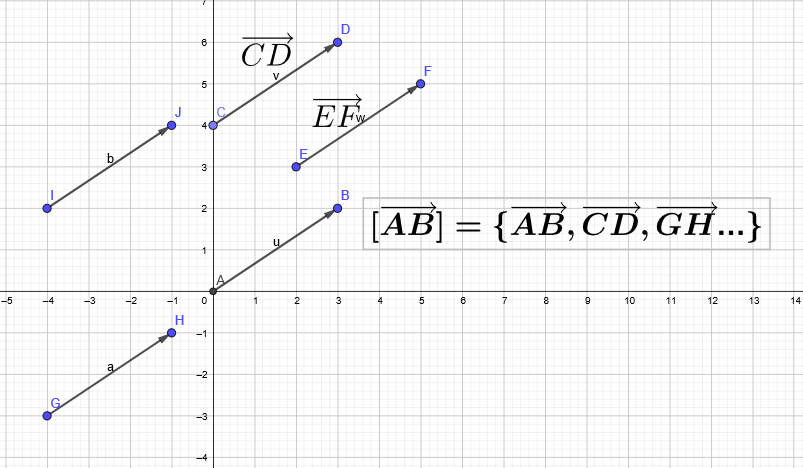
\includegraphics[width=0.9\textwidth]{img/Fijos-libres.png}
    \caption{Los diferentes vectores fijos de $V^2$ que tienen las mismas coordenadas forman parte del vector libre. 
    \newline
    De la misma manera que la idea $\rfrac{1}{2}=\rfrac{2}{4}=\rfrac{3}{6}$ se escribiría formalmente: $\left[\rfrac{1}{2}\right] = \left\{\rfrac{1}{2},\rfrac{2}{4},\rfrac{3}{6} ... \right\}$}
    \label{fig:plano}
\end{figure}


Denotaremos por $[\vec{AB}]$ al vector libre cuyas coordenadas son las del vector que va de $A$ a $B$.

Denotaremos por $\vec{AB}$ al vector fijo que va de $A$ a $B$.





\begin{defn}[Vector\IS definido por dos puntos]
(Página 278)

Dados dos puntos $A=(a_1,a_2,a_3)$ y $B = (b_1,b_2,b_3)$, tenemos 
    \begin{itemize}
        \item $\vec{AB} = \hide{(b_1-a_1, b_2-a_2, b_3-a_3)}$
        \item $\vec{BA} = \hide{(a_1-b_1, a_2-b_2, a_3-b_3)}$ 
    \end{itemize}
\end{defn}

\begin{proof}
Lo único que tenemos para trabajar son vectores de posición. 
%
En este caso son $\vec{a} = \vec{OA}$ y $\vec{b} = \vec{OB}$. 

Tenemos que $\vec{a} + \vec{AB} = \vec{b} \dimplies \vec{AB} = \vec{b}-\vec{a}$.
\end{proof}

\begin{example}
    Halla un vector definido por $A(1,0,3)$ y $B(2,1,2)$.
    
    \hide{\[\vec{AB} = (2-1, 1-0, 2-3) = (1,1,-1)\]}

    \obs Fíjate bien, por favor, que la operación realizada \textbf{no} es una resta de puntos.
\end{example}

\begin{problem}

Utilizando vectores de posición, demuestra que el punto medio entre los puntos $A$ y $B$, que llamamos $M_{AB}$, tiene por coordenadas:

\[M_{AB} = \left(\frac{a_1+b_1}{2},\frac{a_2+b_2}{2},\frac{a_3+b_3}{2}\right)\]

\ppart \textbf{Ampliación:} Dados los puntos $A(a_1,a_2,a_3)$ y $B(b_1,b_2,b_3)$, calcula las coordenadas del punto que divide el segmento $AB$ dejando $\rfrac{1}{3}$ de distancia con $A$ y $\rfrac{2}{3}$ de distancia con $B$. \textit{Pista: planteamiento parecido al punto medio.}

\solution

\[
\left\{
\begin{array}{c}
    \vec{AM} + \vec{MB} = \vec{AB}\\
    \vec{AM} = \vec{MB}\\
    \vec{OM} = ?
\end{array}\right\}
 \implies 
  2\vec{AM} = \vec{AB} \dimplies
  \]\[ 
  2\left(\vec{OM} - \vec{OA}\right) = \vec{AB} \dimplies
  2\vec{OM} = \vec{AB} + 2\vec{OA} = 
  \]\[
  2\vec{OM} = \left(
  b_1-a_1,
  b_2-a_2,
  b_3-a_3
  \right) + 
  \left(
  2a_1 - 0,
  2a_2 - 0,
  2a_3 - 0
  \right) = 
  \left(
  b_1+a_1,
  b_2+a_2,
  b_3+a_3
  \right)\]\[
  \vec{OM} = \left(
  \frac{b_1+a_1}{2},
  \frac{b_2+a_2}{2},
  \frac{b_3+a_3}{2}
  \right)
\]

\end{problem}

% \begin{problem}

% Dado el punto definido por el vector de posición $\vec{OP} = (1,1,1)$ en el sistema de referencia $\{(1,0,0), \mathcal{B} = \{u_1 = (1,0,1), u_2 = (0,2,1), u_3 = (0,0,4)\}\}$, expresa sus coordenadas en el sistema de referencia: 
% %
% $\{(1,1,0), \mathcal{B} = \{\vec{i},\vec{j},\vec{k}\}\}$

% \solution

% ¿Qué significa $\vec{OP} = (1,-2,3)$? Las coordenadas son los coeficientes de los vectores de la base, por lo tanto:

% \[
% P = (1,0,0) + 1·u_1 - 2·u_2+ 3·u_3  \dimplies (1,0,0) + 1·(1,0,1) - 2·(0,2,1)  + 3·(0,0,4) = (2,-4,11)
% \]

% Expresamos el vector $(2,-4,11)$ en el sistema de referencia pedido:

% $(2,-4,11) = (1,1,0) + \lambda_1\vec{i}+ \lambda_2\vec{j}+ \lambda_3\vec{k} \implies (\lambda_1,\lambda_2,\lambda_3) = (1,4,11)$

% \end{problem}

\begin{problem}

Dado el punto definido por el vector de posición $\vec{OP} = (1,1,1)$ en el sistema de referencia $S_1 = \{O_1(1,0,0), \mathcal{B} = \{u_1 = (1,0,1), u_2 = (0,2,1), u_3 = (0,0,4)\}\}$, expresa sus coordenadas en el sistema de referencia: 
%
$S_2=\{O_2(1,1,0), \mathcal{B} = \{\vec{i},\vec{j},\vec{k}\}\}$

\solution

En realidad $\vec{OP} = \vec{O_1P}$, por estar expresado en ese sistema de referencia. 

Entendemos que $O_1(1,0,0)$ no está expresado en función de la base de $S_1$.

¿Qué significa $\vec{O_1P} = (1,1,1)$? Las coordenadas son los coeficientes de los vectores de la base, por lo tanto, tomando $O(0,0,0)$ tenemos:

\[
\vec{OP} = \vec{OO_1} + \vec{O_1P} = (1,0,0) + 1·u_1 + 1·u_2+ 1·u_3  \dimplies\]
\[ (1,0,0) + 1·(1,0,1) +1 ·(0,2,1)  + 1·(0,0,4) = (2,2,6)
\]

Expresamos el vector $\vec{OP}=(2,2,6)$ en el sistema de referencia pedido:
\[\vec{OP} = (2,2,6) = (1,1,0) + \lambda_1\vec{i}+ \lambda_2\vec{j}+ \lambda_3\vec{k} \implies (\lambda_1,\lambda_2,\lambda_3) = (1,1,6) = \vec{O_2P}\]

\vspace{-0.3cm}
\paragraph{Plan b:} 
\[\vec{OP} = \vec{OO_2} + \vec{O_2P} \dimplies \vec{O_2P} = \vec{OP} - \vec{OO_2} = \underbrace{(2,2,6)}_{\ast} - \underbrace{(1,1,0)}_{\Delta} = (1,1,6)\]
\obs Para este planteamiento es \textbf{necesario} que los vectores que operamos (en este caso $\ast$ y $\Delta$) en coordenadas estén expresados en la \textbf{misma base}. 
%
En este caso, dicha base es la base canónica.

\vspace{-0.3cm}
\paragraph{Plan c: } No es necesario pasar por el origen $O(0,0,0)$, aunque pueda resultar más fácil de interpretar así. 

Podríamos haber empezado desde el principio haciendo un razonamiento parecido al plan b. Buscamos $\vec{O_2P}$ y sabemos $\vec{O_1P}$, por lo que podemos plantear:

\[
  \vec{O_1O_2} + \vec{O_2P} = \vec{O_1P} \dimplies \vec{O_2P} = \vec{O_1P} - \vec{O_1O_2}
\]

Como para poder hacer operaciones de vectores en coordenadas necesitamos la misma base, tenemos:

\[
  \vec{O_2P} = \vec{O_1P} - \vec{O_1O_2} = (\textcolor{red}{1},\textcolor{blue}{1},\textcolor{green}{1})_{S_1} - (0,1,0)_{SH} = (\textcolor{red}{1}\vec{u_1} + \textcolor{blue}{1}\vec{u_2} + \textcolor{green}{1}\vec{u_3}) - (0,1,0)
\]\[
  = 1·(1,0,1) +1 ·(0,2,1)  + 1·(0,0,4) - (0,1,0) = (1,1,6)
\]

\begin{itemize}
   \item $(0,1,0)_{SH}$ quiere decir "el vector $(0,1,0)$ expresado en el sistema de referencia habitual".
   \item $(1,1,1)_{S_1}$ quiere decir "el vector $(1,1,1)$ expresado en el sistema de referencia $S_1$".
 \end{itemize} 
\end{problem}


\subsection{La recta}

\obs Dado que la única manera que tenemos de determinar los puntos es a través de vectores de posición, utilizaremos $\vec{p} = (x,y,z)$ de forma equivalente a $[\vec{OP}]$ para referirnos a un punto cualquiera del espacio, al que accedemos a través de su vector de posición.

Formas de determinar una recta:
\begin{enumerate}
  \item Un punto\footnote{O su vector de posición} y un vector director.
  \subitem 2 puntos (se reduce al caso anterior)
  \subitem Un punto y una condición de paralelismo (se reduce al primer caso)
  \item 2 planos secantes.
  \item Un punto y un plano perpendicular (se verá en geometría euclídea).
\end{enumerate}

Como todo con lo que vamos a trabajar son operaciones con vectores con coordenadas en un sistema de referencia, en realidad el punto de origen del sistema de referencia no es relevante. (Ver ejemplo \ref{example::origen_ref}).

\subsubsection{Ecuaciones de la recta}

La 
%
\concept[Ecuación de la recta\IS vectorial]{ecuación vectorial de la recta} $r$ determinada por el punto $A$, cuyo vector de posición es $\vec{a}$, con vector director $\vec{u_r} $  es $r : \vec{p} = \vec{a} + \lambda \vec{u_r}$, con $\lambda\in\real, \forall P\in\real$ (ver \fref{fig::recta_ecuacion_vectorial})
%
De esta manera quedan determinados los vectores de posición de todos los puntos de la recta $r$.


\begin{figure}[hptb]
    \centering
    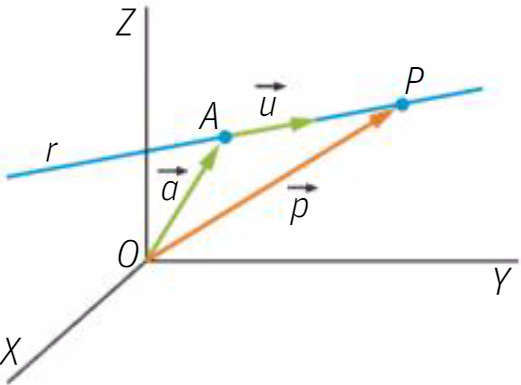
\includegraphics[width=0.4\textwidth]{img/EcVectorialRecta.png}
    \caption{Representación gráfica de la ecuación vectorial de la recta.}
    \label{fig::recta_ecuacion_vectorial}
\end{figure}


¿Es posible construir la recta sin ese parámetro $\lambda$? En realidad,
$$\underbrace{r : \vec{p} = \vec{a} + \lambda \vec{u_r}}_{(0)}\dimplies \underbrace{r:\displaystyle \left\{
\begin{array}{c} 
  x = a_1 + \lambda u_1\\
  y = a_2 + \lambda u_2 \\ 
  z = a_3 + \lambda u_3
\end{array}\right\}}_{(1)} \implies \underbrace{r:\frac{x-a_1}{u_1} = \frac{y-a_2}{u_2} = \frac{z-a_3}{u_3}}_{(2)}$$

\begin{itemize}
    \item A $(1)$ lo denominamos \concept[Ecuación de la recta\IS paramétrica]{ecuación paramétrica de la recta}
    \item A $(2)$ lo denominamos \concept[Ecuación de la recta\IS continua]{ecuación continua de la recta}
\end{itemize}

\[
\frac{x-a_1}{u_1} = \frac{y-a_2}{u_2} = \frac{z-a_3}{u_3}\overset{(1)}{\implies} \left\{
\begin{array}{c}
     \displaystyle\frac{x-a_1}{u_1} = \frac{y-a_2}{u_2}\\
     \displaystyle\frac{y-a_2}{u_2} = \frac{z-a_3}{u_3}
\end{array}\right\} \implies
\underbrace{\left\{\begin{array}{cccc}
     Ax + &By    &     & = D\\
          &B'y   &+ C'z  & = D
\end{array}\right\}}_{(2)}
\]



Donde:
\begin{itemize}
    \item (1) \hide{Se han elegido estas 2 parejas, pero podrían haberse elegido otras, dando lugar a otras ecuaciones implícitas de la misma recta.}
    \item (2) \hide{\concept[Ecuación de la recta\IS implícita]{ecuación implícita de la recta}}
    \subitem \obs \hide{Si interpretáramos las ecuaciones implícitas de la recta como un sistema de ecuaciones, tendríamos un sistema compatible indeterminado con grado de libertad 1.}
    \subitem \obs La dimensión de la recta es 1. \emph{¿Como el grado de indeterminación? Guau...}
\end{itemize}

\begin{problem}
    \ppart 
    Halla todas las ecuaciones de la recta que pasa por $A(0,1,2)$ y es paralela a la que pasa por $B(1,-2,-1)$ y $C(1,0,0)$
    \ppart 
    Halla un vector director de la recta $r:\displaystyle\frac{x-2}{1} = \frac{y-3}{5} = \frac{z-1}{4}$
    \ppart 
    Halla un vector director de la recta $r:\displaystyle\left\{\begin{array}{c} 2x+3y=4\\2x-y+3z=0\end{array}\right\}$
    \solution

\end{problem}

\textbf{Deberes:} 
\begin{itemize}
  \item Página 279.13,14.
  \item Página 281.18-21.
\end{itemize}

\subsection{El plano}

\subsubsection{Ecuaciones del plano}

Un plano queda determinado por \hide{un punto y dos vectores linealmente independientes}

La 
%
\concept[Ecuación del plano\IS vectorial]{ecuación vectorial del plano} 
%
$\pi$ determinada por el punto $A$ y los vectores linealmente independientes $\vec{V_{\pi}}$ y $\vec{W_{\pi}}$  es $r : \vec{p} = \vec{A} + \lambda \vec{V_{\pi}} + \mu\vec{W_{\pi}}$, con $\lambda\in\real$ (ver ). De esta manera quedan determinados los vectores de posición de todos los puntos del plano.

Como en el caso de la recta, podemos escribir esta ecuación en forma de sistema con parámetros:

$$\pi : \vec{p} = \vec{A} + \lambda \vec{V_{\pi}} + \mu\vec{W_{\pi}}\dimplies \underbrace{\pi:\displaystyle \left\{\begin{array}{c} x = a_1 + \lambda v_1 + \mu w_1\\y = a_2 + \lambda v_2 + \mu w_2 \\ z = a_3 + \lambda v_3 + \mu w_3 \end{array}\right\}}_{(1)} $$

 A $(1)$ lo denominamos \concept[Ecuación del plano\IS paramétrica]{ecuación paramétrica del plano}

\[
\pi:\displaystyle \left\{
\begin{array}{c} 
x - a_1 = \lambda v_1 + \mu w_1\\
y - a_2 = \lambda v_2 + \mu w_2 \\ 
z - a_3 = \lambda v_3 + \mu w_3 
\end{array}\right\}
\]
Como los vectores $\vec{v},\vec{w}$ son linealmente independientes y el vector $AX$ es una combinación lineal de los otros 2 (ver \ref{fig:plano}), tenemos:

\[
\left|
\begin{array}{ccc} 
x - a_1 & v_1 & w_1\\
y - a_2 & v_2 & w_2 \\ 
z - a_3 & v_3 & w_3 
\end{array}\right| = 0
\]

Desarrollando esta ecuación, tendríamos una ecuación del tipo $Ax+By+Cz + D = 0$, que llamamos \concept[Ecuación del plano\IS implícita]{Ecuación implícita del plano}.


\begin{figure}[hptb]
    \centering
    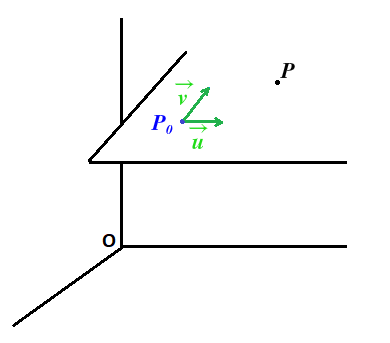
\includegraphics[width=0.65\textwidth]{img/ecplanos.png}
    \caption{Plano generado por un punto y dos vectores}
    \label{fig:plano}
\end{figure}

\begin{problem}
    \textbf{Calcula las ecuaciones del plano que pasa por los puntos $A(1,1,1), B(2,2,2), C(1,2,3)$}

    \solution 

    \hide{
    El primer paso sería calcular 2 vectores linealmente independientes de estos 3 puntos, para comprobar que los 3 puntos forman un plano (y no una recta).

    $\vec{AB} = (1,1,1) \quad\quad \vec{AC} = (0,1,2)$, que son linealmente independientes al no ser proporcionales.

    Ecuación vectorial: $\pi: \vec{p} = (1,1,1) + \mu\vec{AB} + \lambda\vec{AC}, \lambda,\mu\in\real$

    Ecuación paramétrica: $
    \displaystyle\left\{ \begin{array}{c}
      x = 1 + \mu\\
      y = 1 + \mu + \lambda\\
      z = 1 + \mu + 2\lambda
    \end{array} \right\}\text{ con } \lambda,\mu\in\real$

    Ecuación implícita: 

    \[
      \displaystyle \begin{vmatrix}
      x - 1 & 1 & 0\\
      y - 1 & 1 & 1\\
      z - 1 & 1 & 2\\
    \end{vmatrix} = 0 \dimplies \cdots \dimplies x - 2y+z=0
    \]
    }
\end{problem}


\begin{problem}
\ppart Halla la ecuación de 2 rectas que pertenezcan al mismo plano.
\ppart Halla un vector director del plano: $\pi_1: x+y+z = 3$
\ppart Halla el plano paralelo a $\pi_2: x+y+z = 3$ que pase por el origen de coordenadas.
\ppart Halla el plano paralelo al $XY$ que pasa por $A(-1,2,-2)$.
\obs Llamamos plano $XY$ al plano "del suelo", es decir, al plano $z=0$.

\ppart Página 283, ejercicios 25-28.

\solution

\end{problem}

\subsection{Posiciones relativas}

\subsubsection{Entre 2 planos}  

\begin{framed}
\textbf{Ecuaciones vectoriales o paramétricas:}
  \begin{itemize}
    \item Si 2 planos comparten 3 puntos, entonces son el mismo plano.
    \item Si los 4 vectores directores de los 2 planos son linealmente independientes, entonces los planos son secantes en un punto.
    \item Si la matriz formada por los 4 vectores directores de los 2 planos tiene rango 3, los planos son secantes en una recta.
    \item Si la matriz formada por los 4 vectores directores de los 2 planos tiene rango 2, los planos son paralelos.
    \item Si 2 planos paralelos comparten un punto, entonces son coincidentes.
  \end{itemize}
\end{framed}



\subparagraph{Ecuaciones implícitas}

\[
\left\{\begin{array}{c}
\pi_1: Ax+By+Cz = D\\
\pi_2: A'x+B'y+C'z = D'
\end{array}\right\}
\]

Obtenemos las matrices: $M = \displaystyle\begin{pmatrix}A&B&C\\A'&B'&C'\end{pmatrix}$ y $M^* = \displaystyle\begin{pmatrix}A&B&C&D\\A'&B'&C'&D'\end{pmatrix}$

\begin{framed}
  \begin{itemize}
    \item $Rg(M) = Rg(M^*) = 1 $\hide{ coincidentes.}
    \item $Rg(M) < Rg(M^*) = 2 $\hide{ paralelos.}
    \item $Rg(M) = Rg(M^*) = 2 $\hide{ secantes.}
  \end{itemize}
\obs En realidad, sería como las ecuaciones implícitas de la recta.
\end{framed}

\subsubsection{Entre 3 planos}

\subparagraph{Ecuaciones vectorial o paramétricas}

Se pasa a implícitas.

\subparagraph{Ecuaciones implícitas}
\[
\left\{\begin{array}{c}
\pi_1: Ax+By+Cz = D\\
\pi_2: A'x+B'y+C'z = D'\\
\pi_3: A''x+B''y+C''z = D''\\
\end{array}\right\}
\]

Obtenemos las matrices: 
$M  = \displaystyle\begin{pmatrix}
A&B&C\\
A'&B'&C'\\
A''&B''&C''
\end{pmatrix}
$ y 
$M^* = \displaystyle\begin{pmatrix}
A&B&C&D\\
A'&B'&C'&D'\\
A''&B''&C''&D''
\end{pmatrix}
$

Las posibilidades son: (ver figura \ref{fig:PosicionesRelativasPlanos})
\begin{framed}
  \begin{itemize}
    \item $Rg(M) = Rg(M^*) = 1 $\hide{ SCI, secantes en un plano [grado de indeterminación 2, por lo que hay dos parámetros. \textbf{Coincidentes}.}
    \item $Rg(M) < Rg(M^*) = 2 $\hide{ paralelos.}
    \item $Rg(M) = Rg(M^*) = 2 $\hide{ SCI, secantes en una recta [grado de indeterminación 1, por lo que hay un parámetro.}
    \item $Rg(M) = 2 < Rg(M^*) = 3 $\hide{ no se cortan los 3. Sistema incompatible}
    \item $Rg(M) = Rg(M^*) = 3 $\hide{ SCD, secantes en un punto que es la solución del sistema.}
  \end{itemize}  
\end{framed}

\begin{figure}[hptb]
    \centering
    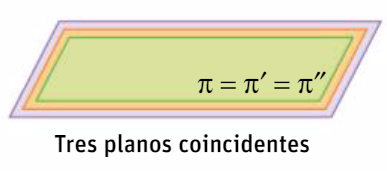
\includegraphics[width=0.65\textwidth]{img/Captura1.png}
    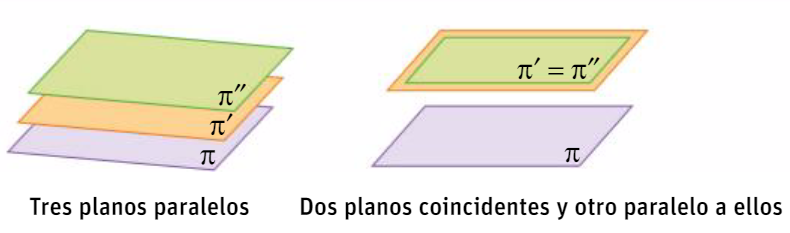
\includegraphics[width=0.95\textwidth]{img/Captura2.png}
    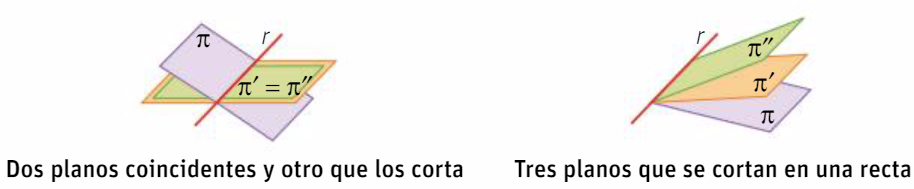
\includegraphics[width=1.1\textwidth]{img/Captura3.png}
    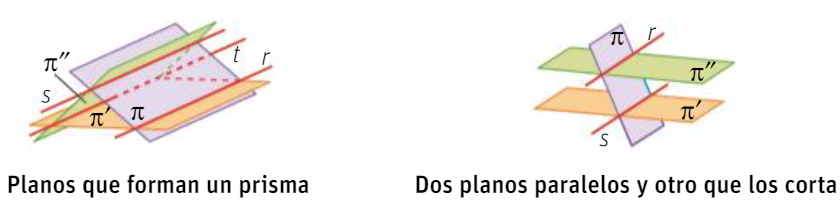
\includegraphics[width=1.1\textwidth]{img/Captura4.png}
    \caption{Representación gráfica de las posiciones relativas de 3 planos.}
    \label{fig:PosicionesRelativasPlanos}
\end{figure}




\subsection{Posiciones relativas entre recta y plano}

\paragraph{Ecuaciones implícitas: } si tanto la recta como el plano están dados en ecuaciones implícitas, estaríamos en la posición relativa de 3 planos, sabiendo que 2 de ellos son secantes en una recta.

\paragraph{Ecuaciones paramétrica: } $\pi: \{P_{\pi},\vec{v_{\pi}}, \vec{w_{\pi}}\}$ 

\begin{center}
\begin{tabular}{ccc}
$P_r \in \pi $ & $\vec{v_r}$ LD de $v_{\pi}, \vec{w}_{\pi}$ & \textbf{Conclusión}\\\hline
No & No & Secantes en un punto\\
No & Sí & Recta paralela\\
Sí & No & Secantes en un punto\\
Sí & Sí & Recta contenida en el plano\\
\end{tabular}
\end{center}

\paragraph{Plano implícito, recta paramétrica: } comprobamos si existe algún valor de $\lambda_{r}$ para el que se cumpla la ecuación implícita del plano. 
\begin{itemize}
  \item $\exists!\lambda \implies $ secante.
  \item $\lambda \in \real \implies$ contenida.
  \item $\not\exists \lambda \implies $ paralela.
\end{itemize}

Deberes: Hoja resumen de teoría,105ab,107ab

\subsubsection{Posiciones relativas entre 2 rectas:}

Dadas las rectas 
$r:\vec{p} = \vec{a} + \lambda\vec{u},\quad \lambda\in\real$
y
$s:\vec{p} = \vec{b} + \lambda\vec{w},\quad \lambda\in\real$. 

Si los vectores directores son paralelos (proporcionales), las rectas pueden ser paralelas o coincidentes. 
%
Para poder distinguir , podríamos ver si un vector formado por un punto de cada recta es también proporcional (entonces serían coincidentes) o si no (entonces serían secantes).

De la misma manera, si los vectores son linealmente independientes las rectas pueden cruzarse o cortarse. 
%
Para distinguir estos 2 casos, podríamos ver si un vector formado por un punto de cada recta es linealmente dependiente a los otros 2 (entonces serían secantes porque formarían un plano que contiene al vector) o si no (entonces se cortarían en el espacio).

Así, buscamos estudiar la dependencia lineal de los 2 vectores directores ($\vec{u},\vec{w}$) y de los 2 vectores directores respecto de un vector formado, arbitrariamente, con 2 puntos de las rectas ($\vec{AB}$, con $A(a_1,a_2,a_3)\in r$ y $B(b_1,b_2,b_3)\in s$). 
%
Para ello, formamos las matrices:

$M  = \displaystyle\begin{pmatrix}
u_1&w_1\\
u_2&w_2\\
u_3&w_3
\end{pmatrix}
$ y 
$M^* = \displaystyle\begin{pmatrix}
u_1&w_1&b_1-a_1\\
u_2&w_2&b_2-a_2\\
u_3&w_3&b_3-a_3\\
\end{pmatrix}
$

\begin{framed}
  \begin{itemize}
    \item $Rg(M) = Rg(M^*) = 1 $\hide{ SCI, secantes en una recta [grado de indeterminación 1, por lo que hay dos parámetros. \textbf{Coincidentes}.]}
    \item $Rg(M) = 1 < Rg(M^*) = 2 $\hide{ paralelas.} 
    \item $Rg(M) = Rg(M^*) = 2 $\hide{ SCI, secantes en un plano [dimensión 2]. $\vec{AB}$ se puede escribir como combinación lineal de $\vec{u}$ y $\vec{w}$}
    \item $Rg(M) = 2 < Rg(M^*) = 3 $\hide{ se cruzan en el espacio.} 
  \end{itemize}  
\end{framed}
\obs También se podría trabajar con las matrices traspuestas si uno está más familiarizado con estudiar el rango como combinaciones lineales de filas en lugar de columnas.

\begin{problem}
Página 289, ejercicios 52, calculando puntos de cortes
\solution

\end{problem}


\subsubsection{Haz (no se pide en selectividad, así que se salta)}
\paragraph{Haz de rectas paralelas: } cambia el punto, manteniendo fijo el vector. 
\paragraph{Haz de rectas secantes: } cambia el vector (sin ser nunca nulo), mantiene fijo el punto.
\paragraph{Haz de planos paralelelos: } cambia el punto, mantiene los vectores
\paragraph{Haz de planos secantes en una recta: } mantiene un vector y un punto, cambia el otro vector.

\begin{problem}
Tema 11: 56,57,59,60.
\solution
\end{problem}

Deberes: 118,136,143

\subsubsection{Practicamos en general}

Tema 11: 
122,127,130,134,135,136,139,140,143,145,149,150

Tema 11:
\begin{itemize}
  \item Básicos: 83,91,92,93a,98,100,101a,103a,104a,105,106,107d,108
  \item Síntesis: 111-119
  \item Completos: 122-124,127,129-133
\end{itemize}



